\section{Keyword Extraction and Pattern Discovery}\label{sec:offline}
% brief explain
This section describes an offline process of the scoring mechanism for keywords and POIs and pattern discovery from trajectory histories.
\subsection{Keyword Extraction} \label{subsec:KE}
In this subsection, we present how we extract the semantic meaning of the keywords and propose a matched score to describe the degree of connection between keywords and trajectories. The keyword extraction module first computes the spatial, temporal and attribute scores for every keyword $w$ in the corpus. At query time, each query keyword will be matched to the pre-computed score of matching $w$.

\subsubsection{Geo-specific keywords} 
Some tags are specific to a location, which represents its spatial nature.
To quantify the geo-specificity of a tag, an external database identifies geo-terms in the overall tag set and then the tag distribution on the map rates the identified geo-terms. Specifically, to identify name tags, we leverage an external geo-database. In Microsoft Bing services, Geocode Dataflow API (GDA) \footnote{https://msdn.microsoft.com/library/ff701733.aspx} can query large numbers of geo-terms and their representative locations. For a tag $w$, using GDA, we set $GDA(w)$ as 1 if its location is returned, and 0 otherwise. Then, using the geographic distribution of the tags, we can find place-level geo-terms like `Taipei101' in noisy geo-terms. Country-level geo-terms like `USA' and city-level geo-terms like `Seattle' are far more widely distributed on the globe than place-level geo-terms. Thus, we compute the variance $GeoVar(w)$ of the $(latitude,longitude)$ set including a tag $w$. With these features, we define a geo-specificity (\textsf{GS}) score of a tag $w$ as:
\begin{equation}
GS(w) \propto GDA(w)\cdot exp(-GeoVar(w))
\end{equation}
We consider a tag $w$ as a geo-specific keyword if $GS(w)$ is greater than a pre-defined threshold.


\subsubsection{Temporal keywords} \label{subsec:KE.temporal}% time distribution
Some tags are specific to a time interval, which represents its temporal nature. To quantify the temporal-spatiality of a tag, time distribution on a tag rates the identified temporal-terms. Using time distribution of tags, we can find tags associated with a specific time interval like `sunset'. Tags independent of time like `Taipei' are far more widely distributed in time than time-specific tags. Thus, to identify temporal-tags, we compute the variance $TimeVar(w)$ of the creation time of check-ins including a tag $w$. With these features, we define a temporal-specificity (\textsf{TS}) score of a tag $w$ as:
\begin{equation}
TS(w) \propto exp(-TimeVar(w))
\end{equation}
We consider a tag $w$ as a temporal keyword if $TS(w)$ is greater than a pre-defined threshold. Then, given a temporal keyword $w$, we generate a 2-dimensional Gaussian $\mathcal{N}_t(\mu,\sigma^2)$ that models the distribution of the occurring time of $w$ and define the associated time of $w$ as a time interval with up to two standard devations from $\mu$.


\subsubsection{Attribute keywords} \label{subsec:KE.attribute}
To find attribute keywords, we consider tags frequently associated with a POI (TF), while not with so many other POIs (IDF). To quantify the relevance between a tag and a POI, we define a ``document'' as an estimated check-in set $I_{p}$ of $p$. Using this POI-driven knowledge, our scoring conveys the POI semantic information in both TF and IDF.

Specifically, we use three types of frequencies: check-in frequency (\emph{pf}), user frequency (\emph{uf}), and POI frequency (\emph{rf}). Given a tag $w$ and a POI $p$, $pf(I_{p},w)$ is the number of check-ins that have $w$ in $I_{p}$. It is reasonable that a tag is likely to be one of the attribute tags as more check-ins of the POI have the tag. However, some users have the same tags in different check-ins causing overestimation of \emph{pf}. Similarly, $uf(I_{p},w)$ is the number of users that assign $w$ in $I_{p}$. \emph{uf} can control overestimated \emph{pf}. However, we need to filter common tags like `Travel', which also have high \emph{pf} and \emph{uf}.
Given a tag $w$ and a set $p$ of all POIs, $rf(L,w)$ is the number of POIs $p \in L$ having $w$ in $I_{p}$. Consider the $rf$ distribution on the overall tag set. The head may contain tags that would be too generic attributes for all POIs, while tags in the tail (i.e., $rf=1$) are likely not to be attribute terms. With these three types of frequencies, we define an attribute (\textsf{AT}) score of a tag $w$ as:
\begin{equation}
AT(w) \propto \max_{p \in L} \frac {pf(I_{p},w)\cdot uf(I_{p},t)}{rf(L,w)}
\end{equation}
We consider a tag $w$ as an attribute keyword if $AT(w)$ is greater than a pre-defined threshold and $rf(L,w)>1$.


\subsection{Pattern Discovery Methods}
To achieve the ``Where, When, Who'' consideration issue of user demands, the pattern discovery and scoring module defines the ranking mechanism for each POI with global attractiveness, proper visiting time and geo-social influence.

\subsubsection{Determining the attractiveness scores of POIs}
Below, we briefly introduce how to determine the attractiveness scores for POIs by mining the transition pattern.

Given a set of trajectories recorded as a series of check-in points, each check-in point represents a POI, which is denoted by $(latitude,longitude)$.

\begin{figure}[t]
 \centering
 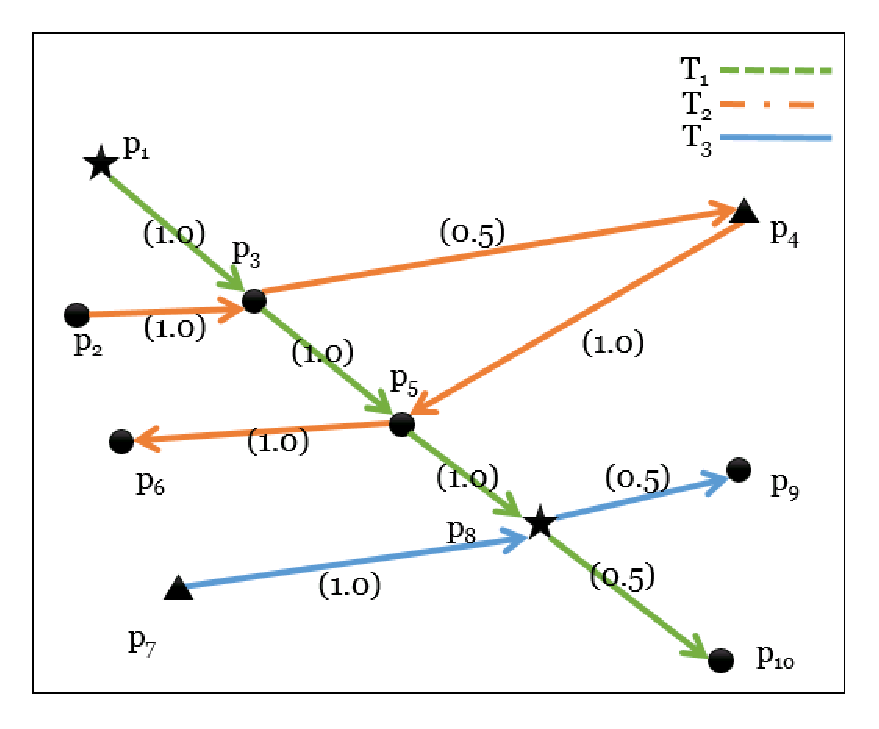
\includegraphics[width=6cm]{RWmodel_TraSearch.eps}
 \caption{An example of a region transition graph}
 \label{fig:RWmodel_TraSearch}
 \end{figure}

To measure the attractiveness of POIs, we intend to explore the sequential relationships hidden in the trajectory records. A region transition graph is built based on the transition probabilities to derive the traversal relationship. The example in Figure~\ref{fig:running_example} can be revised to a region transition graph shown as Figure \ref{fig:RWmodel_TraSearch}. The edges indicate the transition relationships among POIs. The weight of each edge is derived by aggregating the transition relationship from a set of trajectories. With the region transition graph, we borrow the concept in PATS \cite{PATS} to adopt the Markov model to assign an attractiveness score to each POI and denote the attractiveness score of POI $p_{i}$ represented as $AS(p_{i}$). According to PATS~\cite{PATS}, the attractiveness of a trajectory can be inferred by a sequence of POIs and the concept of random walks. % Based on this intuition, we developed a travel trajectory recommendation system for retrieving some interesting routes which fulfill two requirements: (i) travel routes should contain all those query points specified (ii) travel routes should within the spatial range $Q$.


\subsubsection{Proper visiting time decision} \label{sec:offline.2}
As claimed in~\cite{hsieh2012exploiting}\cite{hsieh2014mining}, the pleasure of visiting the POIs along a route is closely related to the arrival time. Some places have a wider range of visiting time period while others are constrained to certain particular time slots. For example, most people do not go to night markets in the morning, but rather arrive in the evening after the market opens. Thus, we extract time information from the timestamp of check-ins and mine the proper visiting time period of each POI. As shown in Figure \ref{fig:time_distribute}, each POI has a different time distribution curve. For example, the distribution of Shihlin Night Market in Figure \ref{fig:night} shows that most people have check-ins during the evening and we can infer that the proper visiting time of Shihlin Night Market is about 17:00 to 23:00. Another example in Figure~\ref{fig:day} shows that most people visit Shilin Presidential Residence during the daytime so the proper visiting time may be 7:00 to 17:00. When the distribution curve approaches a horizontal line, it indicates that the POI is suitable to be visited at any time. On the contrary, when the distribution curve has a peak segment, it indicates that the POI may be popular at a special time and proper to visit at that time. The same concept can be used in the case of seasons, weekends and weekdays.

Here we separate one day into 24 time intervals. We first define the probability of a POI $p$ be visited at time $t$ as ${N(p,t)}/N_{total}(p)$, where ${N(p,t)}$ is the number of people who have check-ins in $p$ at time $t$, and $N_{total}(p)$ is the total number of people who visit $p$. Due to the concern of data sparsity, we apply the 2-dimensional Gaussian $\mathcal{N}_t(\mu,\sigma^2)$ to fit the distribution of visiting time, which is similar to the idea of the temporal score in Section~\ref{subsec:KE.temporal}.
\begin{equation}
P(p,t)=\frac {1}{\sqrt{2\pi}\sigma} exp\left[ -\frac { { \left( x-\mu  \right)  }^{ 2 } }{ 2{ \sigma }^{ 2 } }  \right] 
\end{equation}

After defining the visiting probability, we define the visiting time score $VS(p,t)$ for POI $p$ at time $t$ between 0 and 1 as:
\begin{equation}
VS(p,t)=\frac{P(p,t)}{max_{t\in{0{\rightarrow}23}}(P(p),t)}
\end{equation}
where $max_{t\in{0{\rightarrow}23}}(P(p),t)$ is the maximum probability of visiting $p$ in one day.

\begin{figure}[t]
\centerline{
\mbox{
    \subfigure[Shihlin Night Market]{
        \label{fig:night}
        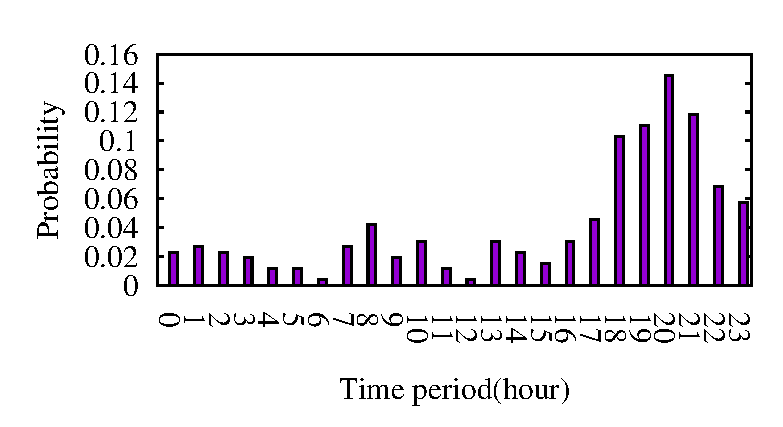
\includegraphics[width=0.55\linewidth]{Shihlin_night_market.eps}
    }
    \subfigure[Shihlin Residence]{
        \label{fig:day}
        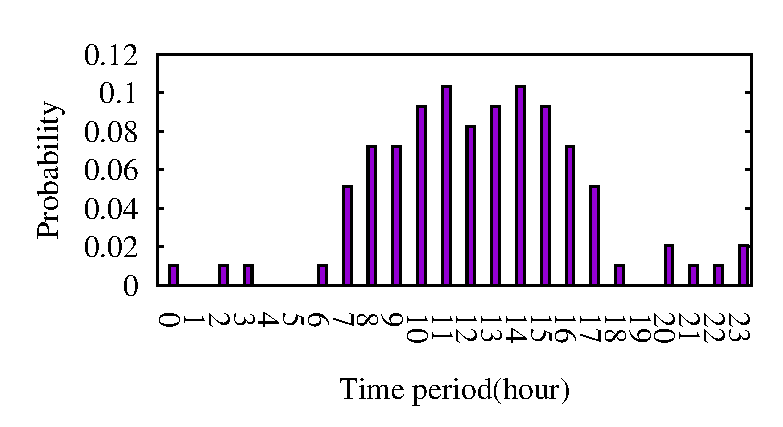
\includegraphics[width=0.55\linewidth]{Shihlin_Residence.eps}
    }
}}
\caption{The distributions of the visiting probability at each time unit (hour) for (a)Shihlin Night Market, and (b)Shilin Presidential Residence from check-in records.}
\label{fig:time_distribute}
\end{figure}

Now we give an example to illustrate how to compute $VS$. Given a visiting time Gaussian distribution of $p$ in Figure \ref{fig:time_ex}, the maximum visiting time probability of $p$, i.e., $max(P(p))$ is 0.08 at the 19:00 time interval, the probability of the 10:00 interval is 0.04, and $VS(p,10)=0.04/0.08=0.5$.

% need to revised! %%%%%%%%%%%%%%%
\begin{figure}[t]
\centering
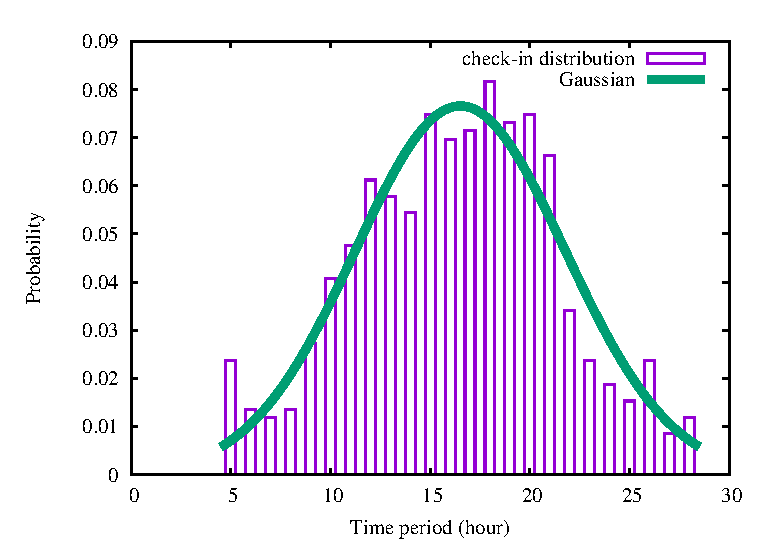
\includegraphics[width=0.8\linewidth]{time_ex.eps}
\caption{An example of visiting time scoring. Two-dimensional Gaussian distribution is adopted to deal with inconsistent data due to data sparsity.}
\label{fig:time_ex} % 一定要在 caption 之後
\end{figure}

\subsubsection{Geographical social influence}
Another important feature in POI recommendation is the social influence of each user. The closer the relationship between two users, the more reliable the recommendation is. We focus on the condition that if user $u_i$ is socially influenced by user $u_j$, $u_i$ would visit a POI because of the recommendation from $u_j$. We can observe a relation that $u_i$ checks in at the same POI $p$ after $u_j$ shared her/his check-in. \cite{ytwen2014} proposed a Social Influence Recommender (SIR) framework to explore the influential users in an LBSN. The main issue is to capture the interaction among the social network, physical locations and time effect by defining the geo-social following relation among users. Then a diffusion model is utilized to stimulate the influence spreading process. The example in Figure~\ref{fig:running_example} can also be revised to Figure \ref{fig:sir_example} to measure the geo-social influence among users.

\begin{figure}[h]
\begin{center}
\begin{tabular}{ccc}

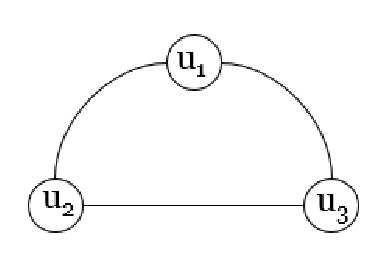
\includegraphics[scale=0.5]{sir_1.eps} &
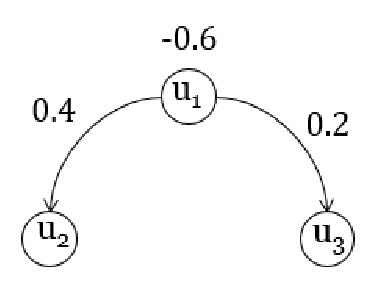
\includegraphics[scale=0.5]{sir_2.eps}
\\
(a) Social graph & (b) Following graph
\\
\multicolumn{2}{c}{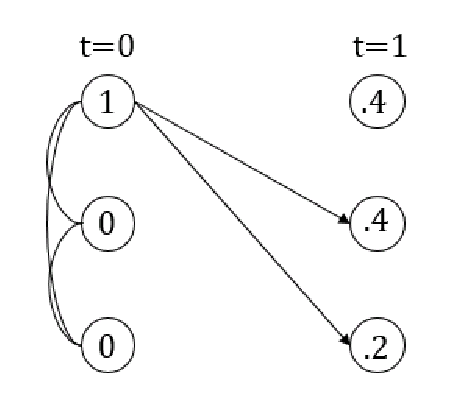
\includegraphics[scale=0.5]{sir_3.eps}}
\\
\multicolumn{2}{c}{(c) Influence propagation from t = 0 to t = 1}

\end{tabular}
\end{center}
\vspace{-3mm}
\caption{An example of influence propagation among three users.}
\label{fig:sir_example}
\end{figure}

The social influence can propagate among the users within the \textit{following graph}. Formally, the amount of influence transited from ${u_i}$ to ${u_j}$ is defined as ${f_{ij}=\frac{p(u_i,u_j)}{n(u_i)}}$. ${p(u_i, u_j)}$ denotes the probability of geo-social following relationships of ${u_i}$ to ${u_j}$, and ${n_i}$ denotes the total number of locations ${u_i}$ has visited. \cite{ytwen2014} assumes that user ${u_i \in V}$ is only influenced by her/himself initially and the influence will be propagated to others in the  \textit{following graph} afterwards. During the propagation process, users receive stimulation from their neighbors. Finally, vector ${s(t)}$ denotes the proportion of the social influence score on users in $V$ at time $t$, the change at ${u_i}$ between time ${t+\Delta t}$ is defined by the following equation using the diffusion model:
%since the first $\textit{follow}(C(u_i,l,t),u_j,\delta)$ happened

\begin{equation}\label{eq:diffusion}
\frac{s(t+\Delta t)-s(t)}{\Delta t}=\alpha Inf s(t)
\end{equation}

where ${\alpha}$ is the propagation coefficient and $Inf$ is a matrix which defines the one-hop information diffusion process. 
